% options:
% thesis=B bachelor's thesis
% thesis=M master's thesis
% czech thesis in Czech language
% english thesis in English language
% hidelinks remove colour boxes around hyperlinks

% arara: xelatex: { shell: yes }
% arara: makeglossaries
% arara: biber
% arara: xelatex: { shell: yes }
% arara: xelatex: { shell: yes }
\documentclass[thesis=M,english,hidelinks]{template/FITthesisXE}

\bibliography{library.bib}
\usepackage{import}
\usepackage{booktabs}
\usepackage{dirtree}
\usepackage{xevlna}
\usepackage{lscape}
\usepackage{float}
\usepackage{nameref}
\usepackage{algorithm}
\usepackage{algpseudocode}
\floatstyle{plaintop}
\restylefloat{table}

\setcounter{tocdepth}{2}

\usepackage[utf8]{inputenc}
\usepackage{graphicx}
\usepackage[export]{adjustbox}

\setlength{\fboxsep}{0.005pt}
\newcommand{\tmpframe}[1]{\fbox{#1}}
%\renewcommand{\tmpframe}[1]{#1}


\usepackage{ifxetex}
\ifxetex
  \usepackage{fontspec}
%  \setmainfont{Linux Libertine O}
\fi

\makeatletter
% fix latex's habit of resetting ' during \write
\begingroup
\obeylines\obeyspaces%
\catcode`\'\active%
\gdef\@resetactivechars{%
\def^^M{\@activechar@info{EOL}\space}%
\def {\@activechar@info{space}\space}}%
\endgroup

% by egreg at https://tex.stackexchange.com/questions/218939/automatic-apostrophes-for-quotation-marks
\renewcommand{\cftchapteraftersnumb}{\hskip1sp\relax}
\let\ORIM@sect\M@sect
\def\M@sect#1#2#3#4#5#6[#7][#8]#9{%
  \ORIM@sect{#1}{#2}{#3}{#4}{#5}{#6}[\hskip1sp\relax#7][\hskip1sp\relax#8]{\hskip1sp\relax#9}%
}
\catcode`'=\active
\protected\def'{%
  \ifvmode
    `%
  \else
    \ifmmode
      \expandafter\expandafter\expandafter\active@math@prime % for math
    \else
      \relax
      \ifdim\lastskip=1sp
        `%
      \else
        \ifdim\lastskip>0pt
          `%
        \else
          \rq
        \fi
      \fi
    \fi
  \fi
}
% redefine \pr@m@s to look for an active '
\def\pr@m@s{%
  \ifx'\@let@token
    \expandafter\pr@@@s
  \else
    \ifx^\@let@token
      \expandafter\expandafter\expandafter\pr@@@t
    \else
      \egroup
    \fi
  \fi}
\makeatother

% from https://www.herout.net/blog/2017/03/pomalu-uz-pojdme-psat/
\usepackage{xcolor}
\newcommand{\todo}[1]{
    \textcolor{red}{\textbf{[[#1]]}}
}
\usepackage{blindtext}
\newcommand{\blind}[1][1]{
    \textcolor{gray}{
        \Blindtext[#1][1]
    }
}

% from https://github.com/Sanqui/fedorator-thesis
\newcommand{\importsvg}[1]{
    \def\svgwidth{\columnwidth}
    \import{media/svg/}{#1.pdf_tex}
}

% usage: \imagefigure{filename}{description}
\newcommand{\imagefigurefull}[3]{
    \begin{figure}[htbp]
    \centering
        \includegraphics[width=#3\linewidth]{media/#1}
        \caption{#2 \label{pic:#1}}
    \end{figure}
}

\newcommand{\imagefigurelarge}[2]{
    \imagefigurefull{#1}{#2}{.99}
}

\newcommand{\imagefigure}[2]{
    \imagefigurefull{#1}{#2}{.6}
}

\newcommand{\screenshotfigure}[2]{
    \imagefigurefull{#1}{#2}{.4}
}

\newcommand{\twofiguresonpage}[2]{
    \imagefigurefull{#1}{#2}{.83}
}

\newcommand{\svgfigure}[2]{
    \begin{figure}[htbp]
    \centering
        \importsvg{#1}
        \caption{#2 \label{pic:#1}}
    \end{figure}
}

\usepackage{amsthm}

\theoremstyle{definition}
\newtheorem{definition}{Definition}[section]

\theoremstyle{remark}
\newtheorem*{remark}{Remark}

\makeglossaries
\newacronym{DP}{DP}{Dark Pattern}
\newacronym{HTTP}{HTTP}{Hyper Text Transfer Protocol}
\newacronym{HAR}{HAR}{HTTP Archive}
\newacronym{HTML}{HTML}{Hyper Text Markup Language}
\newacronym{CSS}{CSS}{Cascading Style Sheets}
\newacronym{API}{API}{Application Programming Interface}
\newacronym{HDBSCAN}{HDBSCAN}{Hierarchical Density-Based Spatial Clustering of Application with Noise}
\newacronym{BoW}{BoW}{Bag of Words}
\newacronym{PCA}{PCA}{Principal Component Analysis}
\newacronym{URL}{URL}{Uniform Resource Locator}
\newacronym{CSV}{CSV}{Comma-separated Values}
\newacronym{DOM}{DOM}{Document Object Model}
\newacronym{L-BFGS}{L-BFGS}{Limited Memory Broyden–Fletcher–Goldfarb–Shanno algorithm}
\newacronym{SGD}{SGD}{Stochastic Gradient Descent}


\glsaddall	% add even unused acronyms

\acknowledgements{I wish to express my sincere thanks to my supervisor, doc. Ing. Tomáš Vitvar, Ph.D., for the continuous encouragement and advice given while writing this thesis.

Furthermore, I would like to thank my whole family, especially my parents, for raising me up and supporting me during my studies. Additionally, I would like to thank my friends. I would like to point out my friend David Whalan making me lose worries in spoken English and my other friend Ing. Tomáš Hodek for encouraging in my life decisions.}
\abstractEN{This thesis investigates patterns in user interfaces, also known as dark patterns, that force users to do things or make decisions differently than they originally intended. This thesis focuses on the detection of dark patterns used by webshops on the Czech Internet and the detection is done on a large scale.

This thesis builds on research already conducted at Princeton University that investigated dark patterns on English webshops.

Several tools were created to retrieve a significant number of webshops. Also the tools from the conducted research were modified to be applied to the Czech language.

These tools were used to obtain multiple datasets mapping webshops on the Czech Internet and the dark patterns used on them.

It was found that dark patterns are widely used on Czech webshops.}
\abstractCS{




% Tato bakalářská práce se zabývá možnostmi využití evolučních algoritmů pro~generování grafických rozhraní na základě uživatelových preferencí. Tato grafická rozhraní mohou být popsána gramatikou, což je sada pravidel, která umožňuje popsat všechna jejich možná nastavení.

% Dalším cílem je využítí zjištěných znalostí k vytvoření prototypu, který bude generovat grafové vizualizace nad danými datasety.

% Na vytvořeném prototypu byly provedeny měření počtu iterací na~vytvoření požadované vizualizace. Jelikož jsou interaktivní evoluční algoritmy závislé na náhodě a~na uživatelových preferencích, nelze jasně říci, že by počet dosažených iterací měl vyšší vypovídající hodnotu. Tudíž měření slouží spíše jako proof of~concept.
}

\title{Detection of Dark Patterns on Czech Webshops}
\authorGN{Petr}
\authorFN{Hanzl}
\authorWithDegrees{Bc. Petr Hanzl}
\author{Petr Hanzl}
\supervisor{doc. Ing. Tomáš Vitvar, Ph.D.}
\keywordsCS{Temné vzory, Automatizované procházení webu, Interakce člověk-počítač, Shluková analýza, Webové obchody}
\keywordsEN{Dark patterns, Web crawling, Human-computer Interaction, Cluster analysis, Webshops}
\department{Department of Software Engineering}
\placeForDeclarationOfAuthenticity{Prague}
\declarationOfAuthenticityOption{5}
\website{https://github.com/Lznah/DarkPatterns}
\assignment{assignment.pdf}

\begin{document}

\begin{introduction}
    Dark patterns\cite{dark-patterns-brignull, dark-patterns-colin, the-year-dark-pattern-won, dark-patterns-at-scale} are ways of designing a user interface of websites, apps or any other computer system in a specific way to trick, confuse or coerce a user in doing unwanted actions like confirming to share more information than is needed to use the service, signing up for things that the user did not mean to, buying unwanted products and more. 

Typically, when the user reads a website or uses an app, he does not read all the words and makes quick assumptions\cite{dark-patterns-brignull}. Dark patterns then trick the user by hiding information of unpleasant truth. The user also trusts in his experience that he has gained from using other websites or apps and expects specific actions to happen or not to happen by using a similar pattern in the user interface. The user is tricked here by excepting this user interface behaviour, but in reality, it does something more or less than what the user expects\cite{the-year-dark-pattern-won}. Dark patterns are not only able to take advantage of the user not paying enough attention. Another dark pattern uses psychological methods to make users feel bad and guilty for not doing what the dark pattern wants them to do\cite{the-year-dark-pattern-won}.

Research into tricky user interface designs and deceptive practices has surprisingly much history, but it was neglected for many years. In 1999, Hanson and Kysar were the first who examined how companies abuse customers' cognitive limitations and profit from them. The rapid growth of the Internet and e-commerce increased more serious discussions and analyses of this topic. The term Dark Pattern itself was introduced by user interface expert Harry Brignull in 2010 to create a library of different types of dark patterns and to shame websites using them\cite{dark-patterns-brignull-about-us}. 

% https://www.darkpatterns.org/about-us

In March 2021, the state of California added new regulation that now bans dark patterns that prevent users from opting out of the sale of their personal data\cite{california-bans-dark-patterns}. Therefore, the topic of dark patterns becomes more and more relevant.

% https://www.theverge.com/2021/3/16/22333506/california-bans-dark-patterns-opt-out-selling-data

In 2019, a group of scientist from Princeton University introduced an automated approach that enables experts to identify dark patterns used on websites at scale\cite{dark-patterns-at-scale}. 

% https://arxiv.org/pdf/1907.07032.pdf

This thesis's primary goal is to build on top of their research to analyse the prevalence of dark patterns on Czech webshops, also described in the Princeton study\cite{dark-patterns-at-scale}. This thesis focuses on product pages and product purchase flow only because these are the most promising pages, where all the buying happens. Several subgoals need to be done to fulfil the primary goal:
\begin{itemize}
    \item Build an automated mechanism of gathering data from numerous Czech webshops at scale.
    \item These extracted data needs to be analysed in order to train a model that can detect dark patterns.
    \item Evaluate and describe results.
\end{itemize}

The thesis does not aim to study the prevalence of deceptive dark patterns that display transients values over time.
\end{introduction}

% \chapter{State of the art}
Most studies \cite{dark-patterns-brignull} \cite{dark-patterns-colin} \cite{taxonomies-conti} in the field of dark patterns have only described known existing types of dark patterns. Also, literature often proposes different dark pattern taxonomies. To find these patterns, scholars did manual research, analyzing page by page.

In contrast to this approach, that requires a lot of manual work, there is a study from Princeton University \cite{dark-patterns-at-scale} and it proposes a completely new taxonomy. Not only the researchers recategorized and made more accurate the currently known types from the literature, but they were able to find new types of dark patterns, thus they extended the literature about these new types.

Princeton researchers also notes that only textual information on webshops were analysed. Continues, that the set of found dark pattern is restricted in this manner \cite{dark-patterns-at-scale}.

To find these new types, reseachers focused on product pages of webshops, because as they say, these pages are the most promising to contain dark patterns at any level of purchase flow \cite{dark-patterns-at-scale}. Princeton Researchers did a lot of work to find these dark patterns. They separated it into three steps as it can be seen in figure \ref{pic:dark-patterns.pdf}.

\imagefigurefull{dark-patterns.pdf}{Overview of the shopping website corpus creation, data collection using crawling, and data analysis as proposed by Princeton University researchers\cite{dark-patterns-at-scale}.}{1}

\textbf{Corpus Creation} is the first step, there are several programmes to get domain names of webshops. They gathered websites with the highest Alexa Rank via Alexa Rank API. Then, they used paid service Webshrinker to filter out only those websites that are webshops. The list of domain still contained non-English websites. They used polyglot language classifier to filter them out of the list. Overall, researches gathered a list of 19K English shopping websites\cite{dark-patterns-at-scale}.

\textbf{Data Collection} is the second step. It consist of two crawlers created by the Princeton researches. The first crawler is meant to find product links on a single website. To speed up the process of finding these product pages, they trained a classifier of Logistic Regression on a dataset of 1000 URL links manually labeled by the researchers. The first crawler found 53K pages in 11K domain names.

The second crawler, also refered as 'checkout crawler', is meant to simulate user's shopping flow. This means that the crawler is able to follow the steps of the buying process - which includes selecting product options (e.g., size or color), adding the product to the card, viewing the cart and checking out. To evaluate, whether or not this crawler is able to simulate user's shopping flow, the researchers randomly sampled 100 product pages and examined whether the crawler successfully reached the checkout page.

This crawler is build on OpenWPN, which is a web privacy measurement framework for privacy studies on a large set of websites\cite{github-openwpm}. Princeton researches implemented additional features to this framework. For example, they created a feature to store HAR files, which contain all the HTTP communication and Javascript calls. All these collected data are further utilized in an analysis phase by researchers. These data help researched to recognize whether or not a found pattern is on of the types of dark patterns.

The checkout crawler also divides visited pages into meaningful textual segments. Researchers propose the definition of this textual segment and an algorithm to split the HTML code of the page into these segments \cite{dark-patterns-at-scale}. Also, the checkout crawler extracts data about text and background colors, positions and dimensions of the segments and others. With this algorithm, there were able to capture approximately 13 million segments across the previously noted 53K product URL pages.

\textbf{Data Analysis} is the last step of the research. It consists of data preprocessing, hierarchical clustering, examining and analyzing the found clusters. The data cleansing phase reduced 90\% of all segments to ~1.3 million segments.

Data were transformed into a representation of Bag of Words (BoW)\cite{bag-of-words}. Then, Principal Component Analysis was performed on the BoW matrix. The outcome were 3 components, which together represented 95\% of the variance in the data. 

Researchers chose an algorithms called Hierarchical Density-Based Spatial Clustering of Application with Noise (HDB-SCAN)\cite{hdbscan} to find clusters in data. They tried different hyper parameters of this clustering algorithm and picked the most promising results.

Then, they did two passes in examining the clusters. In the first pass, they manually tagged clusters that can manifest as dark patterns. This pass reduced the number of the clusters from 10,277 to 1,768. In pass two, they manually examined all the 1,768 clusters, whether the cluster contains any dark pattern \cite{dark-patterns-at-scale}.

Lastly, the researchers discussed the results and they iteratively grouped the discovered dark patterns into categories. They revealed 15 types of dark patterns in 7 categories on 1,254 websites, which represents ~11,1\% out of 10,277 \cite{dark-patterns-at-scale}.





% \chapter{Dark Patterns}
The 'Dark Pattern' is a relatively new term. This neologism was firstly used by Harry Brignull in 2010\cite{dark-patterns-arstechnica} when he registered a domain darkpatterns.org. In this domain, Brignull created an online library to share user interface patterns with deceptive characteristics that intentionally confuse and enrol users in unwanted situations. Another purpose of this online library is to shame websites that use dark patterns.

\section{Definition}
Brignull described dark patterns like so: 'Dark Patterns are tricks used in websites and apps that make you do things that you did not mean to, like buying or signing up for something.'\cite{dark-patterns-brignull} Brignull's definition is simplified to understand what dark patterns with ease. However, it does not include all the dark patterns that Brignull describes. For example, there is a dark pattern that purposely focuses users attention on doing one action and distracts their attention from alternatives. Brignull's definition does not imply this example.

A more accurate definition is the one used in the study made by Princeton researchers. They suggest this definition: 'Dark patterns are user interface design choices that benefit an online service by coercing, steering, or deceiving users into making decisions that, if fully informed and capable of selecting alternatives, they might not make.' \cite{dark-patterns-at-scale}
\section{Taxonomy}

Brignull also defined the first types of dark patterns. This list of types is continuously updated when a new type of dark pattern is found. In April 2021, there were twelve different types of dark patterns defined\cite{dark-patterns-brignull-types}.

The researchers from Princeton University have redefined this list considering the results of their study. This list consists of fifteen types of dark patterns and seven broad categories. Their work also differs from the prior work\cite{dark-patterns-brignull,taxonomies-tales,taxonomies-conti} by the new proposed taxonomy. This new taxonomy focuses on the characteristics of dark patterns and cognitive biases that they exploit in users. They used their taxonomy to classify and describe discovered dark patterns.

This thesis uses the same taxonomy defined by Princeton researchers. This taxonomy consists of five dimensions:

\begin{description}
    \item[Asymmetric] \hfill \\ The user interface presents more alternatives to a user. It is an asymmetric characteristic of a dark pattern if the user interface requires less effort to continue with the alternative that might be disadvantageous for users. A typical example is buttons for accepting and rejecting cookies on websites. Usually, the rejecting button is less noticeable. Also, if users want to reject saving cookies, the user interface forces them to read much more text and click many buttons for every single cookie.
    \item[Covert] \hfill \\ The user interface shows evidence of covert characteristics if users may fail to recognise the intended outcome of a specific action. Users have experience with other user interfaces, and they may predict a similar outcome from the interface that shows similar traits as a decoy to influence their decision-making process. For instance, most of the websites offer a subscription to a newsletter in the process of registration. Usually, this subscription to the newsletter is done by ticking a checkbox in the registration form. When users start to read a sentence mentioning the subscription, they automatically expect that not ticking the checkbox means not subscribing to the newsletter.
    \item[Deceptive] \hfill \\ The user interface induces false beliefs in users by presenting them misleading information. For instance, a website may offer a discount for a limited period of time, but in reality, the discount is permanent. Another example is a website that shows how many users are watching the given product and how many products are in stock. This information can take advantage of the deal by steering users into making quick decisions or inducing false beliefs of the product's exclusivity.
    \item[Hides Information] \hfill \\ The user interface intentionally delay presenting necessary information in places or in time, where or when users do not expect them to be presented. For instance, a website may present extra fees for a bought product at the very last step of the checkout.
    \item[Restrictive] \hfill \\ The user interface restricts the set of choices available to users and takes advantage of it. For example, a website may require to sign up only with Facebook to collect additional personal information.
\end{description}

In addition to these dimensions, Princeton researchers define six different effects on users through exploiting different cognitive biases by specific dark patterns:

\begin{itemize}
    \item \textbf{Anchoring Effect}: The tendency of users to over-rely on the first piece of information in the future decision-making process.
    \item \textbf{Bandwagon Effect}: The tendency of users to value more or believe in something simply because others do.
    \item \textbf{Default Effect}: The tendency of users to stick with default options.
    \item \textbf{Framing Effect}: The tendency of users to choose different options with knowledge of the same information, but with a different way of presenting the options.
    \item \textbf{Scarcity Bias}: The tendency of users to value more things that are more sparse.
    \item \textbf{Sunk Cost Fallacy}: The tendency of users to continue an action because they already invested time or other resources in it. Users tend to continue even if that action is capable of putting them in an even worse situation.
\end{itemize}

\section{Categories and types of Dark Patterns}
The types introduced in this section are the same defined in the paper from Princeton university\cite{dark-patterns-at-scale}. They are based on the types firstly published by Harry Brignull\cite{dark-patterns-brignull}.
Princeton researchers discovered 15 types of dark patterns in total, and they divided them into seven broader categories. The summarisation of these types is in table \ref{tab:darkpatterns} at the end of this section.
    \subsection{Sneaking}
    It is an attempt to hide, disguise, or delay information that is relevant to users. Users would likely change their action future action if they knew about this information. There are three types of dark patterns in this category: Sneak into Basket, Hidden Costs, and Hidden Subscription. Examples of these dark patterns can be seen in figure \ref{figure-examples}
        \subsubsection{Sneak into Basket}
        This type of dark pattern adds additional products into the user's basket without their consent. Usually, he is not aware of this fact. The added products are bonuses or additional services — for example, an additional year of warranty or a gift card. The essential for this dark patterns is that it raises the total price, and users might not be aware of this fact. 
        
        This dark pattern exploits the \emph{default effect} of cognitive bias in users that was described earlier in this thesis. The literature says that this dart pattern is not \emph{covert} because users can see the added products in their baskets.
        \subsubsection{Hidden Cost}
        This pattern is an attempt to add additional charges, typically at the end of the purchase process. Typical examples of this type of dark pattern are additional service fees or handling costs. 
        
        This type of dark pattern is also not \emph{covert}, but it may be considered partially \emph{deceptive} because the information is delayed from users. Also, this dark pattern can be classified into \emph{hides information} dimension, as it attempts to hide information from users.
        \subsubsection{Hidden Subscription}
        This pattern signs up users into a subscription with a recurring fee. Users may not be aware of this subscription because the subscription is presented as a one-time payment or a free trial. This type of dark pattern usually appears together with another dark pattern named 'Hard to Cancel'. 
        
        This dark pattern is classified to be partially \emph{deceptive} because it may confuse and mislead users. Also, it can be said that this dark pattern \emph{hides information} from users.
    \subsection{Urgency}
    Dark patterns from this category speed-up users decision-making process by exploiting scarcity bias in users. For example, this can be done by showing more beneficial or time-limited discounts to users. As a result, users value products more than they would normally do. These dark patterns usually keep signalling that the special offer may be lost to users if they do not react promptly. This dark pattern is usually combined together with 'Social Proof' and 'Scarcity' types of dark patterns defined below. Examples of 'Urgency' dark patterns are shown in figure \ref{figure-examples2}.
        \subsubsection{Countdown Timers}
        This dark pattern is usually in the form of an indicator of a deadline, counting down to the end of the deadline. 
        
        This dark pattern is classified as partially \emph{covert} because it evokes untrue feelings of immediacy in users and is sometimes classified as \emph{deceptive} because the indicator sometimes shows false information. For example, the timer can reset every time it reaches the deadline.

        \subsubsection{Limited-time Messages}
        The 'Limited-time message' dark pattern differs from 'Countdown Timer' by static urgency message and not showing the exact time of the deadline. 
        
        With the taxonomy defined before, this dark pattern is classified as \emph{covert} because of the same reason as 'Countdown Timer' dark pattern and \emph{information hiding} because it does not show the deadline in its offers.
    \subsection{Misdirection}
    This category of dark patterns uses visuals and language to distract users' attention on other possible presented choices. Also, some types from this category use users' emotions to invoke bad feelings of being guilty or ashamed for not making a specific choice. Users trust or feel that the other choices are unavailable or less beneficial for them. Essential for this dark pattern is that other choices are not hidden. Users are aware of the other choices, but this category of dark patterns steers users away from the other choices. Princeton researchers discovered four types of dark patterns from this category: 'Confirmshaming', 'Visual Interference', 'Trick Questions', and 'Pressured Selling'.
        \subsubsection{Confirmshaming}
        The 'Confirmshaming' dark pattern uses language and emotions to focus the attention of users on one choice in order to distract attention on other choices. Researchers point out that this dark pattern usually appeared in popup dialogues that asked for an email address in exchange for a discount. Users who did not want this discount had to choose a button (and the website did not want to choose this button) with the text 'No, I want to pay full price' or 'No thanks, I hate saving money'. This dark pattern exploits the framing effect of cognitive bias in users by presenting choices differently to users.
        
        Thus, this dark pattern is classified as \emph{asymmetric}. However, it is not \emph{covert} since all the possible choices are presented to users.
        % mám něco z alzy

        \subsubsection{Visual Interference}
        The 'Visual Interference' dark pattern uses different styles and visuals to draw users' attention to certain choices - the choices that the website wants users to choose. A typical example of this dark pattern is two buttons in different styles for opting-in and opting-out for the website's newsletter subscription. One of the buttons - the one that the website wants users to click on - looks more promising, more attractive to users' eyes than the other one. The different styles steer users attraction to the opting-in choice. 
        
        By provided taxonomy, this type of dark pattern is partially classified as \emph{asymmetric} because it sometimes unequally present choices to users. Users may not realise that the effect of the dark pattern influenced them. Because of this fact, this dark pattern is also classified as \emph{covert}. Some instances can be also classified as \emph{deceptive}, and Princeton researchers give an example of an option "lucky draw" among others that are deterministic and not random.
        % tady příklady z alzy a z kasa.cz

        \subsubsection{Trick Questions}
        The 'Trick Question' dark pattern uses confusing language to confuse users and their ability to make decisions. A typical trick in the English language for this dark pattern is double negatives. For example, websites, using this type of dark pattern, invert the meaning of a check subscription checkbox, usually seen in registration forms, followed with confusing language 'Uncheck this box if you prefer not to receive email updates'. Users need to pay more attention to properly understand which state of the checkbox means the subscription for the newsletter and which not. This type of dark pattern exploits the default effect in users, who erroneously believe that to them presented user interface follows traditional patterns. Also, this dark pattern exploits the framing effect by presenting the same information in a different, more confusing way to influence users in choosing different choices. 
        
        Therefore, Princeton researchers classify this type of dark pattern as \emph{asymmetric} because opting out takes more effort than opting in. Also, researchers classify this dark pattern as \emph{covert} because users may falsely understand the effect of their choice.
        \subsubsection{Pressured Selling}
        Princeton researchers define the 'Pressured Selling' dark pattern as pre-selecting more expensive variations of the same product as default. Additionally, pressuring users into choosing the more expensive variations or buying related products is also considered as a tactic of this dark pattern. More cognitive biases are triggered and exploited by this dark pattern, such as the default effect, the anchoring effect (users may tend to overlook the other choices) and the scarcity bias (more expensive variations may seem to be more exclusive).  
        
        This dark pattern is for some instances classified as \emph{asymmetric} (i.e., steering users and their acceptance towards more expensive options), and partially \emph{covert} (users may fail to realise that the firstly shown price of the less expensive variation of the product is not the same price, as the more expensive default variation).
    \subsection{Social Proof}
    The 'Social Proof' category of dark patterns is based on a social proof principle. Those hesitating individuals, who do not know what to do in a given situation, tend to observe others and mimic their moves, actions, and behaviour \cite{influence-cialdini, evilbydesign}. This category of dark patterns misuses this behaviour of individuals, and it exploits the bandwagon effect of cognitive bias to its advantage. Princeton researchers define two types from this category: Activity Notifications and Testimonials of Uncertain Origin.

        \subsubsection{Activity Notifications}
        The 'Activity Notifications' dark pattern is information on product pages that indicate other users' activity. The message can have different forms. It can be a number of other users watching the same product or a number of sold products to other users. Messages displaying recent purchases of other users (e.g., 'User X just bought a product Y') also counts as 'Activity Notifications' dark pattern. Princeton researchers point out that some websites claim activity that is deceptive and not true. These websites use a misleading random number instead of factual information. This number also changes after some time, making it even more challenging to recognise as deceptive. 
        
        Some instances of this dark pattern can be classified as \emph{covert} because users fail to understand that this dark pattern influences their decision-making process in a way that they tend to buy a product, which is sold more often or is viewed more by other users. Also, some instances are classified as \emph{deceptive} because they present made up untruthful information and users are not aware of this fact.
        \subsubsection{Testimonials of Uncertain Origin}
        This type of dark pattern refers to the use of customer testimonials whose origin is unclear and not sourced enough. The result of such testimonials is that users' decision-making process is influenced by untrue information, and they erroneously believe in the quality of products.
        
        Using taxonomy defined by Princeton researchers, this dark pattern is classified as sometimes \emph{deceptive}, and it depends on the truthfulness of the testimonials, which can be determined by scanning the website and looking for a submission form for sending testimonials.

    \subsection{Scarcity}
    The 'Scarcity' category contains such types of dark pattern that implement messages indicating limited availability or high demand for a product. Thus, the value of the product increases because of its exclusivity. This dark pattern forces users to make quicker decisions. Users may feel intimidated by losing the chance to buy this very desirable product because it could be sold out soon. Princeton researchers define two types of dark patterns: 'Low-stock Message' and 'High-demand Message'.
        \subsubsection{Low-stock Message}
        The 'Low-stock Message' dark pattern informs users about the limited availability of a product; thus, users want to prevent losing the chance to buy the product by making quicker decisions than they normally do. Some instances of this dark pattern show exact quantities left on the stock. Others only show a message that stock is almost empty. This dark pattern exploits scarcity bias in users - making products more valuable only because it is low on stocks. Some websites use untruthful data to keep arousing the feelings of need in users all the time.

        Princeton researchers classify the 'Low-stock Message' dark pattern as partially \emph{covert} because users fail to realise that these messages influenced their decision-making process. Some instances of this dark pattern are classified as \emph{deceptive} for displaying false information to users about being low on stock, but it is not. Some other instances are classified as \emph{information hiding} for hiding the exact quantities of the product on stock.

        \subsubsection{High-demand Message}
        The 'High-demand Message' dark pattern informs users that a product is in high demand and can be sold out soon.

        Similarly to 'Low-stock Message' dark pattern, 'High-demand Message' is also classified as partially \emph{covert}.

    \subsection{Obstruction}
    This 'Obstruction' category contains only one type of dark pattern, which is 'Hard to Cancel'. This type of dark pattern refers to make specific actions harder to complete than other actions. For instance, signing up for a subscription to an annually paid service is often much more straightforward than cancelling the subscription \cite{unbounce-subscription}. Also, Princeton researchers mention examples when cancellation of a subscription is available only by calling customer service\cite{dark-patterns-at-scale}.

    This dark pattern is sometimes classified as \emph{restrictive} with the defined taxonomy because it restricts the available choices to cancel the previous subscriptions. The 'Hard to Cancel' dark pattern becomes \emph{information hiding} when the website does not inform users how to cancel the subscription or about the fact that cancellation is not as easy as signing up.

    \subsection{Forced Action}
    The 'Forced Action' dark pattern category forces users to take additional action, even though they might not normally take it to finish their task. The 'Forced Enrollment' is the only type of dark pattern discovered and defined by Princeton researchers in this category. This type of dark pattern forces users (that want to use the service) into enrolling for a marketing newsletter or into creating accounts, which gives the website more information than is needed to use the service. Princeton researchers describe an example when users have to simultaneously sign up for a marketing newsletter alongside their consent to terms of service.
    
    Princeton researchers define this type of dark pattern as \emph{assymetric}, because of the requirement of the additional actions to complete users' tasks, which creates asymmetrically balanced choices, and \emph{restrictive}, because it forces users into creating accounts and signing up for marketing newsletters.

\begin{table}
    \centering
    \caption{Summarisation of categories and types of dark patterns with their description, definition and cognitive biases they exploit \cite{dark-patterns-at-scale}.}\label{tab:darkpatterns}
    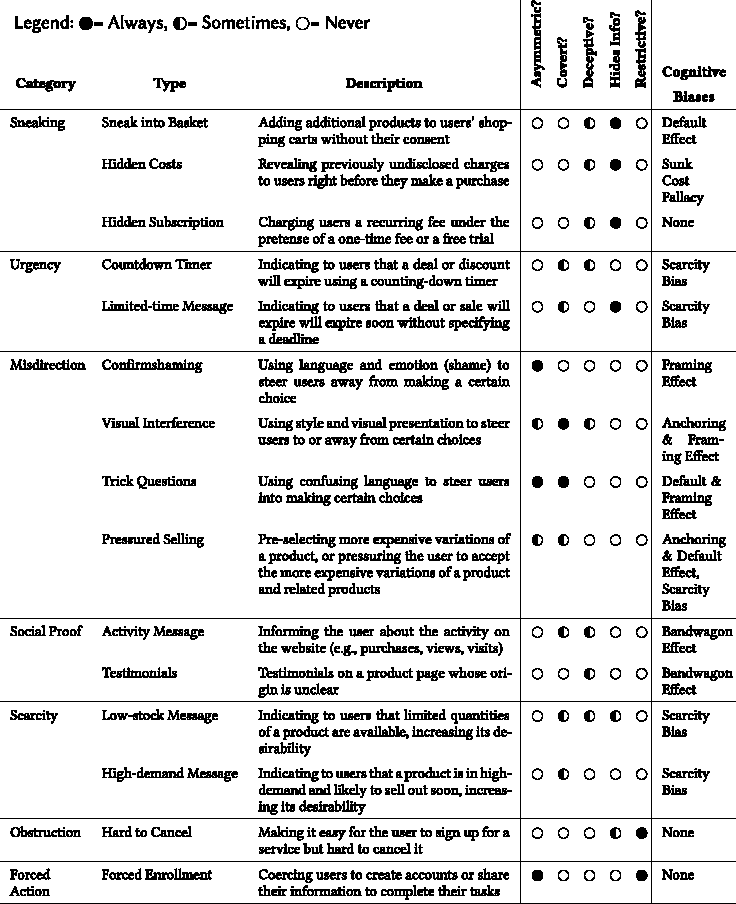
\includegraphics[width=1\textwidth]{media/dp-table.pdf}
\end{table}
% \chapter{Machine Learning}

The term machine learning was firstly coined in 1959 by Arthur Samuel. He described machine learning as: "the field of study that gives computers the ability to learn without being explicitly programmed."\cite{machine-learning-samuel}.

Tom M. Mitchell proposed a new formal definition in 1997\cite{machine-learning-mitchell}, which is:
\begin{definition}
A computer program is said to learn from experience $E$ with respect to some class of tasks $T$ and performance measure $P$, if its performance at tasks in $T$, as measured by $P$, improves with experience $E$.
\end{definition} 

Mitchell also describes an example where a computer program that learns to play chess improves its performance $P$ by gaining experience $E$ from games played against itself. Performance $P$ is measured as the ability to win in a class of tasks $T$, which in this example are the tasks of playing checkers.

\subsection*{A checkers learning problem:}

\begin{itemize}
    \item Task $T$: playing checkers
    \item Performace measure $P$: percent of games won againts humans or other programs
    \item Training experience $E$: percent of games won againts itself
\end{itemize}


Mitchell continues that all learning problems can be specified in this way, such as learning to recognise handwritten words, or learning to drive a robotic automobile autonomously.

\subsection*{A handwritten recognition learning problem:}

\begin{itemize}
    \item Task $T$: recognising and classifying handwritten words in a picture
    \item Performace measure $P$: percent of correctly recognised words
    \item Training experience $E$: a dataset of handwritten words with correct recognition
\end{itemize}

\subsection*{A robot driving learning problem:}

\begin{itemize}
    \item Task $T$: driving on a highway using cameras
    \item Performace measure $P$: average distance travelled before an error occurs
    \item Training experience $E$: a recorded video of a human driver as a sequence of images and steering commands
\end{itemize}

\section{Approaches}

Traditionally, all machine learning tasks can be divided into three broad categories according to the type of feedback provided to the learning system. These are supervised learning, unsupervised learning, and reinforcement learning\cite{ml-types1,ml-types2}.

Reinforcement learning is not described at all in this thesis, as reinforcement learning is not suitable for any type of machine learning problem addressed in the practical part of the thesis.

\begin{figure}[ht]
    \centering
    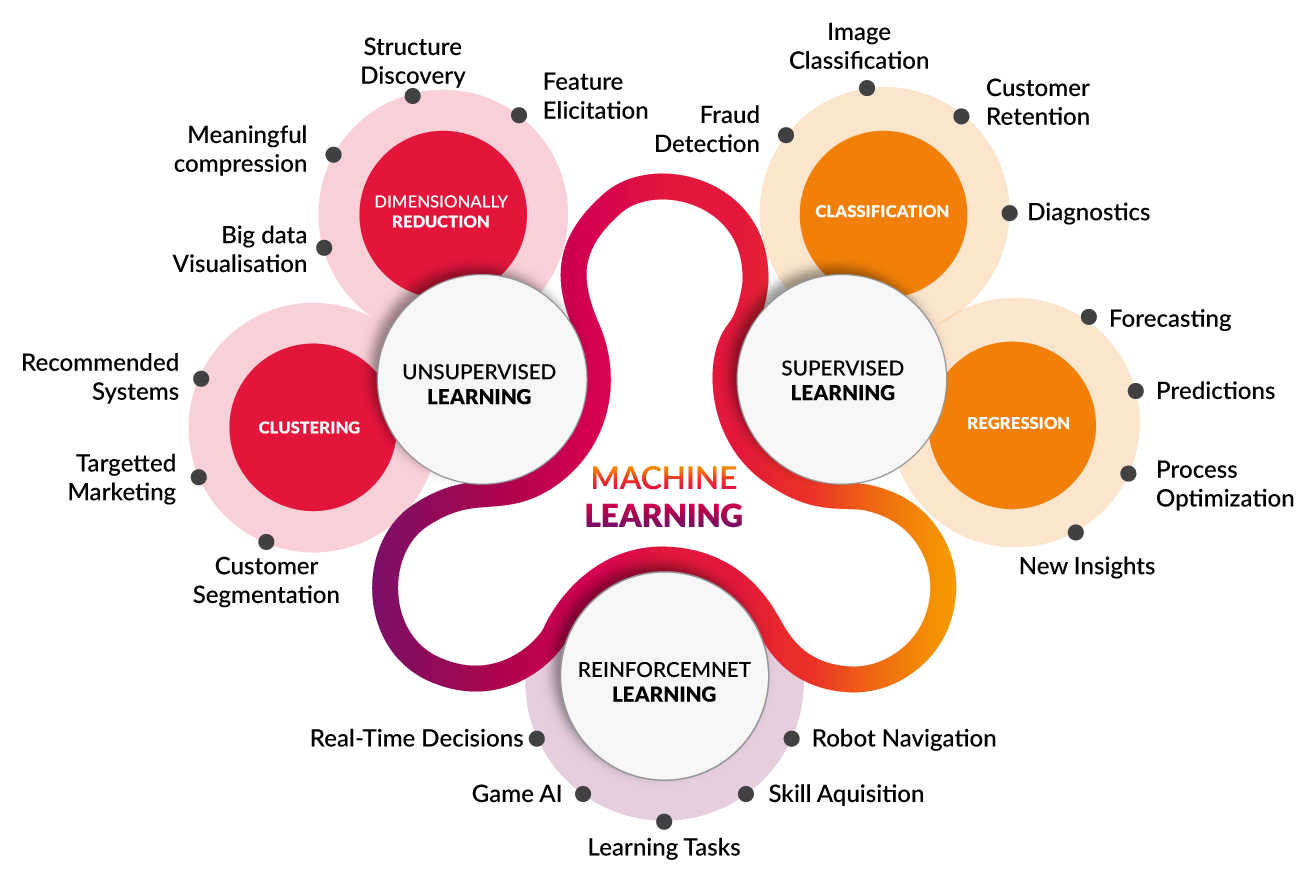
\includegraphics[width=1\linewidth]{media/machine-learning-approaches.png}
    \caption{The three basic learning approaches in machine learning with subcategories and typical applications. The vast majority of machine learning algorithms fall into these three categories.\cite{machine-learning-approaches}}
    \label{fig:machine-learning-approaches}
\end{figure}

Some literature\cite{ml-types1,ml-types2} defines semi-supervised learning, which combines supervised and unsupervised approaches mentioned above, as another learning method. However, since all three basic approaches can be combined, these combinations of learning approaches are omitted in this thesis.

It is also important to mention that the output of a machine learning algorithm, which is usually stored after the learning process and which is subsequently used in the decision-making process, is called a \textbf{model}\cite{algorithms-vs-models}.

\subsection{Supervised learning}

% přidat odkaz na kapitolu logistic regression

In supervised learning, the program is given a dataset that already contains not only what are the input variables, but also what the correct output should look like. Most times, this dataset is created by a person who knows what the correct output should be - a supervisor. Therefore, this type of learning is called as supervised learning.\cite{all-models}

Supervised learning problems are further categorized into two subcategories, classification and regression problems, depending on what the output is\cite{coursera-ml}. If the output is to be a numerical value, such as the price of a property, it is a regression problem. However, if the output is to be whether or not there is a cat in the picture, then it is classification problem. Also, it can be said that algorithms for regression problems are used to predict continues values and algorithms for classification problems are used to predict (or classify) discrete values.

\subsubsection{Regression}
As mentioned earlier, the output of regression algorithms is continuous values. It can be said that a regression solving algorithm looks for a correlation between the input dependent and independent variables. In detail, the input of the learning algorithm is the first pairs of input dependent and independent variables. The algorithm first searches for the mapping function that best captures the unknown correlation in the learning phase. After that, when the algorithm is presented with data for which we do not know the output, the algorithm uses this learned function to predict the value.

A common example of a regression problem is that a machine learning algorithm predicts property prices based on a dataset of properties sold in the past. This dataset contains features such as a number of rooms, location, property condition, and more. It also contains the sale price. Thus, in the learning phase, the algorithm estimates which features lead to which price. Or rather, what is the correlation between the properties of a property and its selling price. Subsequently, this learned model is saved. Then the algorithm is switched to a mode where it no longer learns but returns the property's price depending on what data it is given.

\subsubsection{Classification}

As with regression, the classification algorithm tries to find the correlation between the dependent and independent variables. The learning and subsequent prediction (classification) also work similarly to regression. The output of classification is not a continuous value but a discrete value. 

For example, it can be a decision whether a cancer is malignant or benign. The number of discrete values can be more than one. Also, the output of the classification does not have to always be a logical true-false value for every classification problem. The classification might recognize whether there is a pig, a dog, or a loaf of bread, or even something more in a picture.

\begin{figure}[ht]
    \centering
    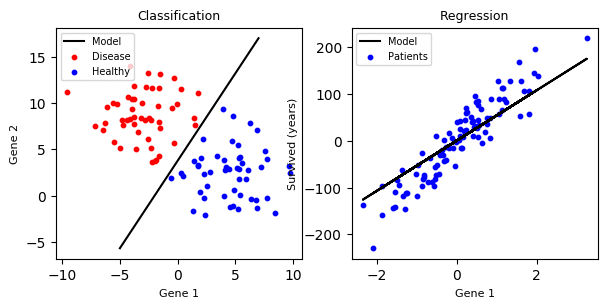
\includegraphics[width=1\linewidth]{media/classification-regression.png}
    \caption{Graph visualization of classification and regression tasks. Classification predicts which set a new patient fits into. Regression predicts the continuous value of the number of years a patient can survive.\cite{classification-regression}}
    \label{fig:classification-regression}
\end{figure}

\subsection{Unsupervised learning}
Unsupervised learning, unlike supervised learning, allows teaching a system without prior knowledge of what the output should look like. This type of learning looks for similarities and patterns in the data instead of mapping input values to labels in the dataset.\cite{coursera-ml}

Unsupervised learning is further divided into two subcategories based on how these similarities and patterns found in the data are used. These subcategories are clustering and dimensional reduction.

\subsubsection{Clustering}

% přidat odkaz na kapitolu HDBSCAN

The goal of clustering is to divide data that are similar into groups\cite{ml-types2}. The number of these groups can be an exact number defined by an expert for some algorithms (K-means\cite{k-means}), but there are also algorithms that find the number of groups by themselves (OPTICS\cite{optics}, DBSCAN\cite{dbscan}.

An example of using clustering methods is recommender systems that recommend the same things to users with similar characteristics to other users. Other examples include anomaly detection, statistical data analysis, and social network analysis\cite{clustering-applications}.

Clustering methods are broadly divided into \textbf{hard clustering} and \textbf{soft clustering}, depending on whether individual data points can fall into only one class (hard clustering) or multiple classes (soft clustering). In the case of soft clustering, each data point is scored with a probability measure that determines which clusters the data point belongs to \cite{clustering-types}. 

\textbf{Types of clustering methods:}
\begin{itemize}
    \item Partitioning Clustering
    \item Density-Based Clustering
    \item Hierarchical Clustering
    \item Grid-Based Clustering
    \item Fuzzy Clustering
\end{itemize}

It is not important for this thesis to describe all these types of clustering methods, except the HDBSCAN method (Hierarchical Density-Based Spatial Clustering of Applications with Noise) used in this thesis's practical part. HDBSCAN is a combination of Density-Based Clustering and Hierarchical Clustering. A detailed description and information about the HDBSCAN method are given in Section XY.

\subsubsection{Dimensional reduction}

% TODO - přidat odkaz na kapitolu PCA

As mentioned earlier, the main task of dimension reduction algorithms is to transform data from a higher dimensional space to a lower-dimensional space\cite{ml-types2}. This is often done during the preprocessing phase of the data, which can be sparse and contain much redundancy. Dimensional reduction algorithms select the interesting parts of the data in the dataset. This also avoids the problem of the curse of dimensionality\cite{bellman1957dynamic}.

Most dimensionality reduction algorithms are further divided into \textbf{feature extraction} or \textbf{feature elimination} algorithms\cite{ml-types2}.

A very commonly used dimensionality reduction algorithm is Principal component analysis, which is also used in the practical part of this thesis and is described in Chapter XX.

\begin{figure}[ht]
    \centering
    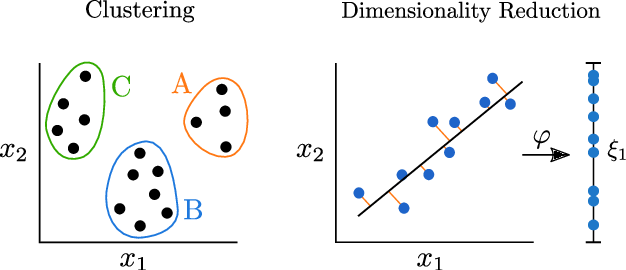
\includegraphics[width=1\linewidth]{media/clustering-reduction.png}
    \caption{Illustration of the output of clustering and dimensional reduction. Clustering searches for patterns among distantly similar data. Dimensional reduction transforms higher dimensional data into lower dimensional data.\cite{clustering-reduction}}
    \label{fig:clustering-reduction}
\end{figure}


% \input{"chapters/04-setup.tex"}
% \chapter{Corpus Creation}

One of the steps of the analysis of the prevalence of the dark pattern on Czech webshops is to find webshops URLs on a large scale autonomously. The Princeton researchers used Alexa Rank\cite{alexa-topsites} made by a web traffic analysis company, Alexa Internet. Alexa Rank is a measure of website popularity. Alexa Internet provides API to fetch a list of most popular websites by Alexa Rank. However, this list contains other types of websites as well, not only webshops that researchers focus on. Also, non-English websites are included as well. Because of that, researchers implemented a couple of mechanisms to cherry-pick English webshops only, discussed earlier in the state-of-the-art chapter of this thesis.

As said before, this thesis aims to analyse Czech webshops and because of that, using Alexa Rank is not efficient enough. Alexa API provides only the first five hundred thousand most popular websites, which is a reason why it contains a small number of Czech websites and even fewer Czech webshops. However, the Czech Internet (that means only websites in the Czech language) is relatively small compared to the English Internet. Also, the English Internet is under multiple jurisdictions, but the Czech Internet is not. Therefore, the Czech Internet is more consistent, and a result of it is that this environment allows creating companies that make Internet catalogues and comparison shopping websites (aggregators) that cover a significant portion of the Czech Internet. 

These catalogues and tools also sometimes rank the listed websites by a measure that has connotations to popularity. For example, a number of testimonials are an excellent resource that reflects the popularity of the webshop. These catalogues and aggregators can be used to mine the URLs of Czech webshops from them instead of using Alexa Rank API. Also, if there is a similar measure as described above, the analysis results can be compared to Princeton's researcher analysis, revealing a correlation of dark patterns evidence on the website and the popularity of the website.

While searching the Internet, several such suitable sites were discovered that contain extensive lists of Czech webshops. Examples of the most suitable sites are Heureka.cz, Asociaceeshopu.cz and Shopy.cz.

Other vital facts that played a role and were considered in the selection of the only one website (that is later used for the creation of the list of Czech webshops) were the actual cover of the Czech Internet. Heureka has by far the highest number of webshops in their listings\cite{srovnavace-shoptet}. However, a few of the biggest webshops do not want to be listed on Heureka. Their reason is usually Heureka itself because it compares the prices of products on the enlisted webshops. Also, Heureka is a part of a business group that runs several competitive webshops. Because of that, the final list (made in this practical part of the study) of Czech webshops was manually checked if it contains the five biggest webshops (according to the list published on website peak.cz\cite{peak-eshopy}), and it does.

\begin{figure}[ht]
    \centering
    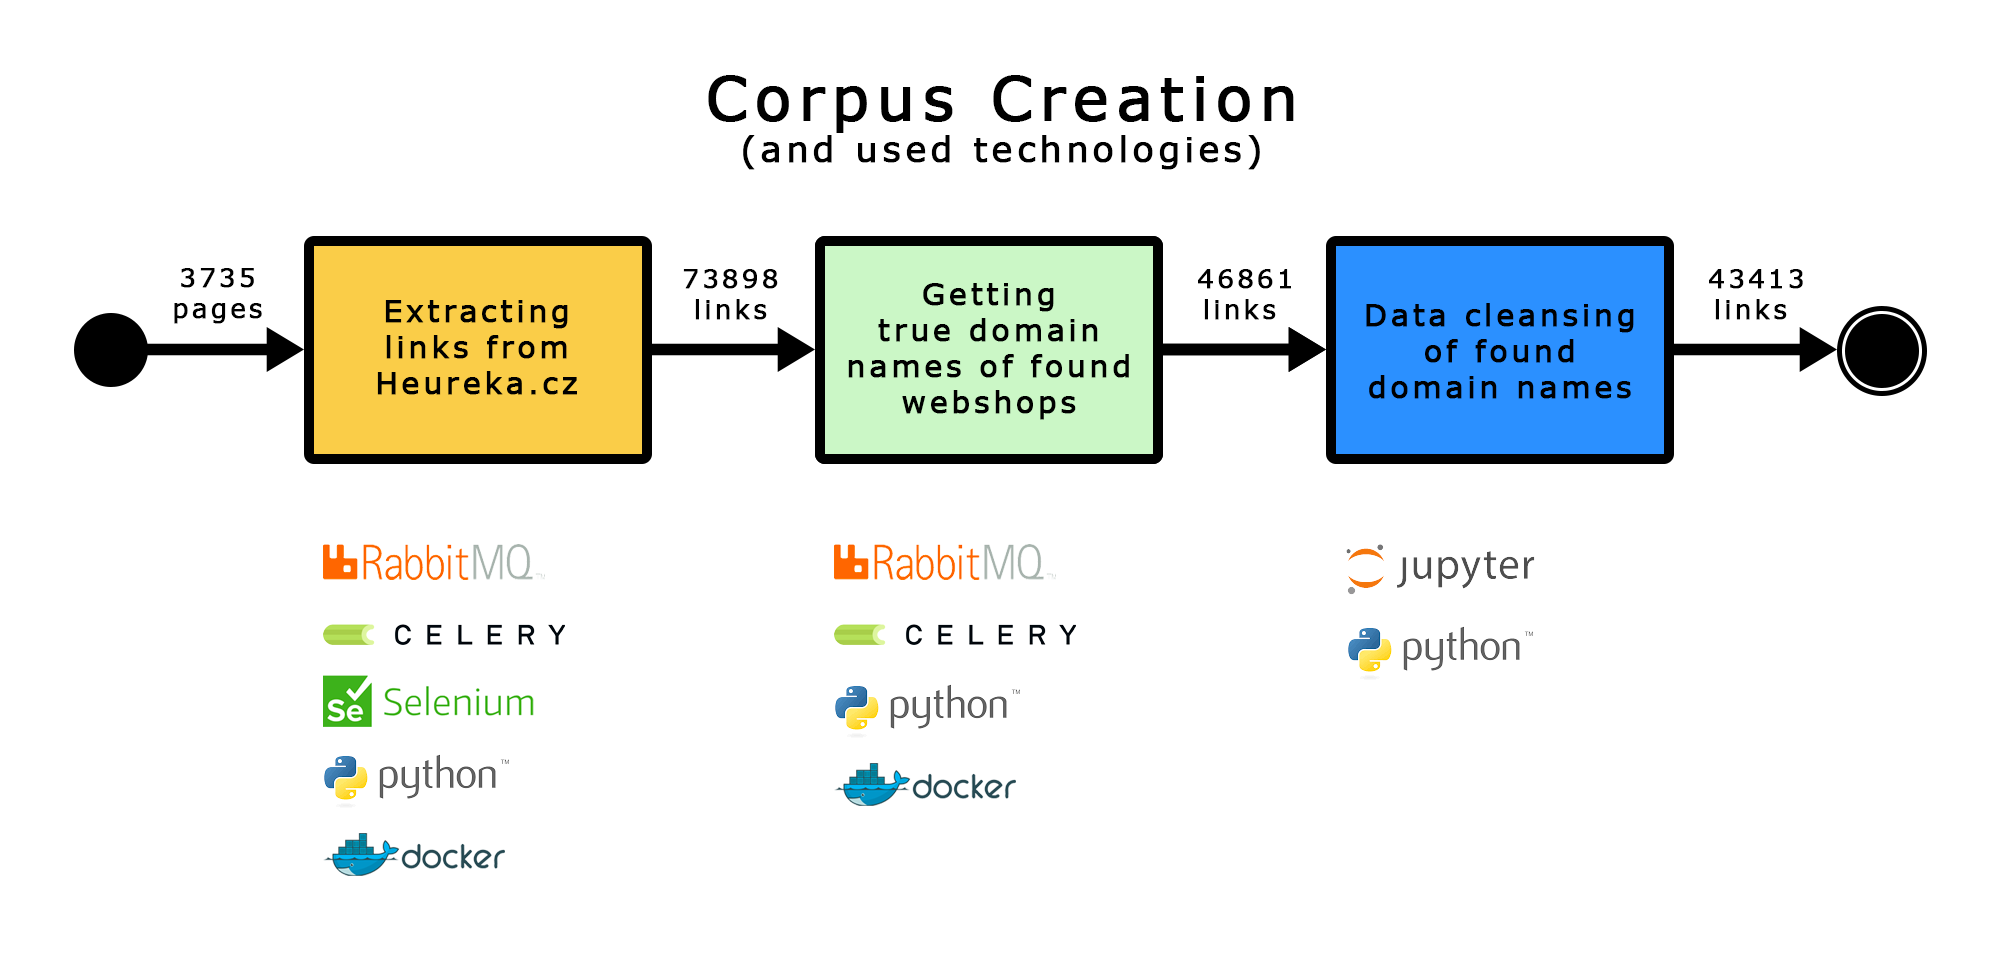
\includegraphics[width=1\linewidth]{media/corpus_creation.png}
    \caption{All steps of corpus creation, which starts with a list of webshops available on Heureka.cz, paginated into 3735 pages and ends with a list of 43413 unique webshops' URLs in CSV format.}
    \label{fig:corpus_creation}
\end{figure}

\section{Extracting webshops from Heureka}

Heureka provides a list of all registered webshops on their website. This list is paginated, where every page contains twenty records of webshops. However, Heureka does not provide the total number of these pages. 

In February 2021, the total number of pages was 3735. This number of pages was manually found by changing the query parameters from the URL until the page stopped returning error 404. At the same time, these 3735 pages contained 74698 webshops in total. 

A web crawler was made to extract webshops' links and names from these pages. The crawler is written in Python 3, using Selenium framework with Chrome browser in headless mode. Also, the crawler is parallelised to speed up this task using Celery asynchronous task queue. Source codes are inside \textbf{src\string/crawler\string/extract\_shops} folder. 

Some of the crawled pages were not successfully downloaded because the Chrome browser occasionally failed to start or the webserver returned an empty page. The crawler was still able to successfully download \textbf{3695 pages} containing \textbf{73898 webshops} in total after scraping the HTML into 3695 CSV files.

Such a high number of obtained webshops does not correspond with the number of webshops that Heureka claims to contain on its homepage (it claims to aggregate around 38000 webshops). Also, the estimated number of webshops on the Czech Internet is around 41000 according to a study made by Zbozi.cz and Shoptet.cz\cite{srovnavace-shoptet}. The cause of this is that the retrieved list of webshops contains many duplicities and already inactive webshops.

Another problem with this list is that the retrieved links are not the actual domain names of the webshops. These URLs are redirections, and they must be visited first to retrieve the actual domain name.

The two other steps of the Corpus Creation deal with these two problems.

\section{Retrieving true domain names}

As mentioned above, Heureka does not provide direct URLs to webshops in its listings. The provided links only redirect to the true URLs of webshops, and because of that, another crawler was made to follow these redirections and return the true URLs. This crawler is also written in Python 3. This time, the task is only to retrieve the true URLs. Hence, Request library is used instead of Selenium, which is too complex for such a simple task. It remains parallelized using Celery. Sources codes are in \textbf{src\string/crawler\string/reveal\_true\_domains} folder.

This crawler adds an additional column to the dataset given from the previous crawler, which contains the true URL. If an exception occurred during the execution of the single task, its message is written there instead. If the webpage returned a different status code than 200, the status code is also written there instead. The importance of this data about errors and exceptions are helpful in the validation of the whole task. Whether the whole task is successful or it returns too many errors and exceptions.

\section{Cleansing of dataset}

The given data from the previous crawler is further cleansed in a Jupyter notebook \textbf{src\string/crawler\string/domain\_dataset\_cleansing.ipynb} using primarily Pandas library.

In the first step, the dataset is split into two data frames of errors and true URLs. Dataset of errors contains 27037 rows, and 23238 of them are results of connection being refused after redirection. The first exception might be that Heureka implemented mechanisms to prevent the crawling of the redirections. This claim was refuted by \textbf{manually going through 100 random} links. None of these links redirects to an active webshop. The next most frequent errors were 404 errors with 1953 occurrences, 403 errors with 750 occurrences and 503 errors with 504 occurrences. These are errors that indicate that the web store web page is no longer active. The other errors had an incidence of fewer than 200 occurrences.

The dataset of true URLs is further cleansed by filtering out other identified inactive webshops that were not identified in the error/rejection filtering. Firstly, such webshops URLs have a high frequency in the dataset because the webshops' URLs are often redirected to the webshops' hosting service website after deactivation of the webshop. For example, many Czech webshops use Shoptet service, which allows users to rent a done webshop solution for a monthly payment. After the users stop paying this fee, their webshop is inactivated (or deleted), making the original webshop be redirected to Shoptet's custom webpage informing visitors about the inactivation of the particular webshop. Secondly, many URLs of inactive webshops contain status code in the URL without sending the actual status code in an HTTP response. Lastly, some domain names were inactive or resold and redirected to a new website (surprisingly redirected to porn websites in most of the cases). All this manual work led to creating a list of such URLs and was used to filter them out of the dataset. This shrinked the dataset from \textbf{46861} to \textbf{46023} rows, removing another \textbf{838} rows.

The last step is to remove URI parts from the URLs and drop duplicate entries, which shrank the dataset to final \textbf{43413} unique links to webshops, removing another \textbf{2610} rows.

Links to download all the outputs and logfiles of crawling are on README page of GitHub repository of this thesis. The link to this repository is in Appendix B (Supplemental Material) of this thesis.

The final list of Corpus Creation stage can be found \textbf{clean\_eshop\_list.csv} in an archive \textbf{reveal\_true\_domains\_crawl\_2021\_02\_23.tar.bz2}.

% dát tam tabulčičku, která to zesumíruje
\chapter{Data Collection}

The second step of the analysis is to find the candidates for dark patterns. This thesis, like the paper on which it is based\cite{dark-patterns-at-scale}, focuses only on a textual representation of dark patterns in terms of finding candidates.

A random sample of one hundred records was drawn from the final dataset from the previous chapter. The URLs from this sample were manually visited, and it was found that the linked page was not a web store for six samples, and thirteen were already non-functional URLs. In addition, it was discovered that the more of these non-compliant URLs mainly were located at lower positions in the dataset. This finding is not surprising, as large web stores last longer and thus are higher in the list of stores.

This sample is updates and user later in data colletion, where records with non-compliant URL are replaced with compliant ones for a total of one hundred records. This sample is saved in \textbf{src/crawlers/extract\_links/list-100-shops.csv}

Looking for the candidates is divided in two steps or two crawlers respectively. The goal of the first step is to find product pages on the webshops in the final list from the chapter Corpus Creation. The goal of the second step is to lookup for the textual candidates on the found product pages and saving them into Redis database for the further analysis.

The two crawlers are based on the crawlers implemented for the original research done at Princeton\cite{dark-patterns-at-scale}. The original crawlers are written in Python 2 and now rewritten into Python 3, since the Python 2 is a deprecated version since January 2020. These crawlers are build in Selenium framework and they use Javascript for the navigation in DOM structure of websites









% Náhodně jsem vybral 100 linků z nichž 6 nebylo eshopem, 13 bylo již nefunkčních. Pravděpodobně čím níže link je, tím menší pravděpodobnost, že bude fungovat. Abych to mohl potvrdit, tak by bylo třeba otestovat více odkazů. Tento list jsem doplnit o nové eshopy, které jsem taktéž ověřil, zda se jedná o eshopy.

% Update:
% Aktualizoval jsem program tak, aby fungoval v Pythonu3.
% Zároveň jsem přidal možnost vyhledávat bez predikce. To jsem dělal kvůli tomu, abych mohl vyhledat seznam linků, které poté určím, že jsou produktové stránky. Nicméně systém nefungoval tak jak jsem myslel a procházel zbytečně moc webových stránek, které evidentně nebyly produktové.
% Program jsem upravil také tak, že jsem přidal různé české varianty a překlady slov a používáných frází, které jsou programem použity na vyhledávání akčních tlačítek jako "Vložit do košíku" a také na filtraci stránek, které zřejmě nejsou produktové (kontakty, o nás, košík atp.)

% Provedl jsem krátný průzkum nejčastěji používaných frází pro vkládání do košíku. Provedl jsem tedy manuální procházení produktových stránek ze seznamu 50 stránek a našel tyto nejčastější fráze:
% 1) Do košíku (19 z 50)
% 2) Přidat do košíku (18 z 50)
% 3) Koupit (7 z 50)
% 4) Vložit do košíku (6 z 50)

% Z tohoto vyplývá, že jediné použité fráze jsou "do košíku" a "koupit". S vyznamností se neobjevují odchylky ve skloňování atp.

% Přidat pak info o tom, na cem to bezelo, jak rychle atp.



% Únor 2021

% Získávání kandidátů na Dark Patterns z produktových stránek:
% - Pro hledání produktových stránek je vytvořený spider, který prochází adresy na doméně a rozpoznává z těchto adres, které adresy jsou produktových stránek. Rozpoznání produktové stránky zajištuje naučený klasifikátor na rozpoznávání produktových stránek.

%     Učení modelu pro klasifikaci produktové stránky:
%     - Tento klasifikátor je naučený v Jupyter notebooku ProductPageClassifier.ipynb. Adresy, které jsou využity pro učení klasifikátoru jsou získány přes jednoduchý spider z náhodných domén v datasetu. Ručně jsou tyto získané adresy ohodnoceny, zda se jedná o produktovou stránku, či nikoliv. 

%     Procházení produktových stránek:
%     - 
% \chapter{Data Analysis}
    Analyzing millions of segments is not optimal for an expert analyst. The work of this expert is expensive and time-consuming. Therefore, methods that reduce the number of segments and thus the expert's work need to be used to make the analysis manageable for the expert. The output is a list of text segments that contain dark patterns.

    The methods used in this section follow the work of the Princeton researchers. At the same time, the results of this work are again compared with the results of their work.

    The data analysis can be divided into four steps:

    \section{Preprocessing}
        The SQLite database, which has 9.5 million segments, contains many duplicate segments across multiple websites. For example, "Add to Cart" buttons, various unified headings such as "Product Description", and others. Since only the text of the segments is analyzed, only those segments that have unique text across a single domain are selected from the dataset for further processing. Also, all the numbers in the dataset have been replaced with placeholders, thus reducing the dataset even more. 

        The output of this preprocessing is a reduction in the number of segments from ~9.5M segments to ~805K. Thus, this approach led to a 92\% reduction in the number of segments. Again, the results are similar to those of the Princeton researchers who achieved a 90\% reduction.

    \section{Feature processing}
        In order to be able to use clustering in the next step, the texts of the segments must first be transformed into a representation for which the similarities between the segments can be expressed mathematically (hereafter, the document means the internal text of the segment).  For this purpose, the Bag-of-Words model is used here. This model is a type of word embedding that represents a document as a string of the number of occurrences of words from a dictionary of all words used across all documents. 

        However, many words do not have only one base form. Especially in the English language, a single word can have many forms due to inflections such as declension and conjugation. The basis of the Bag-of-Words model is the previously mentioned dictionary. If that dictionary contained all the occurrences of the different forms of words, the dictionary would be unnecessarily large and inefficient. For example, the distances of two very similar documents could be disproportionately large simply by rewriting them in a different tense.

        This mischief can be avoided by stemming or lemmatisation, where stemming returns the roots of words. Lemmatization produces the basic forms of words (infinitive for verbs and first-person singular for nouns, adjectives, pronouns and numerals). Lemmatization also considers the context of the word and is, therefore, more accurate\cite{stemming-and-lemmatisation}. On the other hand, it is slower than stemming.

        The Princeton researchers used stemming from the NLTK Python library\cite{nltk}. Still, because both methods (stemming and lemmatisation) depend on the language and because the NLTK library does not support the Czech language, another library had to be chosen.

        Such a library is UDPipe\cite{udpipe} by the Institute of Formal and Applied Linguistics at Charles University. Also, one of the functionalities of this library is tokenisation in the Czech language, which is needed to split the documents into individual words (also referred to as tokens)\cite{tokenisation}.

        Each document is tokenised during the dictionary creation process, producing a list of tokens for which lemmas are obtained and then added to the dictionary. Also, stop words from the Czech language and punction are filtered out of these lists.

        The vocabulary after all the described steps above had a size of \textbf{~269K} tokens. However, this vocabulary still contained tokens, which did have not enough occurrences in the documents.

        Furthermore, only those that appeared in the documents at least 100 times were selected. There were only 188 such tokens. The Count Vectorizer\cite{count-vectorizer} was used to create the BoW matrix, which counts the number of token occurrences in a document. 

        Using Principal Component Analysis (PCA) with 3 retained components on the BoW matrix led to a dimensional reduction which captured 95\% of the variance in the data.

    \section{Clustering}
        The goal of clustering is to group data together. In this case, it means clustering segments into clusters based on similarity. The expert then evaluates the resulting clusters, which makes the expert's job of manual passes easier.

        The clustering method used was HDBSCAN (Hierarchical Density-based Spatial Clustering of Applications with Noise). According to the Princeton researchers, they selected this clustering algorithm because it is robust to noise and, in particular, allows to choose the minimum size of the output clusters.

        In total, HDBSCAN was performed for four different hyperparameter settings. The number of output clusters and the size of the noise cluster was analysed.  The metric used and the minimum cluster size mentioned earlier were the hyperparameters varied. The metrics used were $L_{1}$ and $L_{2}$ norms, also known as Manhattan and Euclidean distance. The hyperparameter of the minimum cluster sizes selected was 5 and 10 segments, which keep the size of noise small and prevents two or more clusters (that are separatable) from forming only one.

        The analysis showed the number of clusters is significantly lower for the models with a minimum cluster size of 10 segments. Similarly, as for the results from Princeton researchers, the difference between selected metric distances was not very significant for data. As expected, models with a larger minimum cluster size have a larger noise cluster size. However, this noise cluster is slightly less than 50\% larger, while the number of all clusters is twice as small. Therefore, a model with a minimum cluster size of 5 segments was selected using the Manhattan distance as the metric with \textbf{4248} clusters (one cluster is the noise cluster). The table \ref{table:hyperparameters-hdbscan} summarised the number of clusters and size of noise for the given hyperparameters. 

        \begin{table}[h!]
            \centering
            \begin{tabular}{r|cr|cr|}
            Minimum cluster size  & \multicolumn{2}{c|}{5}                               & \multicolumn{2}{c|}{10}                              \\ \hline
            Distance metric       & \multicolumn{1}{c|}{L1}    & \multicolumn{1}{c|}{L2} & \multicolumn{1}{c|}{L1}    & \multicolumn{1}{c|}{L2} \\ \hline
            Number of clusters    & \multicolumn{1}{r|}{9040}  & 9088                    & \multicolumn{1}{r|}{4249}  & 4265                    \\ \hline
            Size of noise cluster & \multicolumn{1}{r|}{80980} & 80083                   & \multicolumn{1}{r|}{98436} & 97651                   \\ \cline{1-5} 
            \end{tabular}
            \caption{Number of clusters and size of noise cluster for different distance metrics and minimum size of a cluster.}
            \label{table:hyperparameters-hdbscan}
        \end{table}

    \section{Analysis of output clusters}
    \label{section:analysis-of-output-clusters}
        The clusters that were obtained in the previous step are manually scanned in two steps.

        In both passes, I put myself in the role of an expert who evaluates what is and what is not a dark pattern. I used the knowledge I gained from writing the Dark patterns section. I also used available literature \cite{dark-patterns-brignull-types}\cite{dark-patterns-colin}\cite{kysar-douglas}\cite{taxonomies-tales}\cite{taxonomies-conti}. In uncertainty, I also used the Internet to find out examples what is and what is not a dark pattern, to keep my decisions even more objective. However, the subjective component could still play a role in the decision making process.

        In the first pass, I selected those clusters for which any segment could manifest a dark pattern. For example, the selected clusters were commonly countdowns, total cart prices, user references, notifications, product options, logins and registrations. Only the text components of the segments were checked, not how the segment actually looks on the page. This pass resulted in the number of clusters being reduced from 4249 to 477.
        
        In pass two, I investigate these 477 clusters by directly visiting the website where the dark pattern is searched. If the page no longer exists or does not match the segment, then I investigated screenshots that were obtained during the simulated putchase flow instead. I extended this search by manually going through the entire shopping process directly on the web page and manually searching for all dark patterns.
        
        Lastly, this output dataset of found dark patterns is examined and cleaned from duplicities.
% \input{"chapters/08-results.tex"}

% \begin{conclusion}
%     \input{"chapters/9x-conclusion.tex"}
% \end{conclusion}

% \printbibliography[]


% \appendix

% \chapter{List of Acronyms}
% \printglossary[type=\acronymtype,style=acronyms]

% \chapter{Supplemental Material}

The source code of the thesis and the implementation can be found on the attached medium or online at GitHub.

\noindent \textbf{Thesis} \hfill
    \url{https://github.com/Lznah/master-thesis}

\noindent \textbf{GraphEvolution} \hfill
    \url{https://github.com/Lznah/DarkPatterns}

\vfill

\begin{dirfigure}%
    \dirtree{%
        .1 .
        .1 README.md        \DTcomment{the file with a brief contents description}.
        .1 MT\_Petr\_Hanzl\_2019.pdf \DTcomment{the thesis text in PDF format}.
        .1 DarkPatterns/  \DTcomment{repository for the prototype}.
          .2 src/           \DTcomment{source code of the prototype}.
        .1 thesis/          \DTcomment{the directory of \LaTeX{} source codes of the thesis}.
    }
\caption{Contents of the attached medium}
\end{dirfigure}


\appendix
\chapter{Page segmentation}
\label{appendix:pseudocode}

\begin{algorithm}
    \caption{Page segmentation}
    \begin{algorithmic}[1]
        \State $ignoredElements \gets \textrm{['script', 'style', 'noscript', 'br', 'hr']}$
        \State $blockElements \gets \textrm{['div', 'section', 'article', 'aside', 'nav', 'header', 'footer', 'main', 'form', 'field-set', 'table']}$

        \Function{FindMeshIndex}{$\textrm{position}, \textrm{nGrid}$}
        \EndFunction
    \end{algorithmic}
\end{algorithm}

\end{document}
